% !TEX encoding = UTF-8
% !TEX TS-program = pdflatex
% !TEX root = ../thesis.tex

%************************************************
\chapter{The Effective Higgs Potential \& the Stability of our Universe} \label{chap:3:effective_higgs_potential}
%************************************************

Like all other quantities in the \acs{SM} Lagrangian, the parameters dictating the shape of the Higgs potential~\eqref{eq:2:Higgs_Lagrangian} require renormalization when we go to higher orders of perturbation theory. It was noticed by Coleman and E. Weinberg~\cite{Coleman:1973jx} that these radiative corrections can significantly alter the potential, and by extension the whole \acs{SM}. In the following, we want to investigate the effect of these loop corrections and answer a very important question: is the Higgs potential stable?

As we showed in Section~\ref{sec:2:EW_symmetry_breaking}, the Goldstone bosons are not physical particles since they can be absorbed by a suitable gauge choice. The study of the Higgs potential hence boils down to its dependence on the Higgs field component which is invariant under the gauge transformation. Following our previous convention, this means we only have to consider the real part of the second component of the Higgs field, \ie\ only the real scalar field $\phi = \frac{1}{\sqrt{2}} \text{Re} \Phi_2$. When expressed in terms of this field, the Higgs sector of the Lagrangian becomes
\begin{equation}
\begin{gathered}
\mathcal{L}_H = \frac{1}{2} D_\mu \phi D^\mu \phi - V(\phi) \\
V(\phi) =  \frac{1}{2} \mu^2 \phi^2 - \frac{\lambda}{4} \phi^4.
\end{gathered}
\label{eq:3:Lagrangian_phi}
\end{equation}

One can show that a sufficient condition for \acs{SSB} is that a non-vanishing \acs{VEV} be a stationary point of the effective action
\begin{equation}
\frac{\delta \Gamma [\phi]}{\delta \phi} = 0, \quad \phi \neq 0.
\label{eq:3:SSB_condition}
\end{equation}
Where the effective action is defined as the Legendre transform of the generating functional for connected Green's functions $W[J]$, \ie
\begin{equation}
Z[J] \equiv \mathcal{N} \int \mathcal{D} \phi \, e^{i (S[\phi] + J \cdot \phi)} = e^{i W[J]} = e^{i (\Gamma[\phi] + J \cdot \phi)}, \quad \phi \equiv \frac{\delta W}{\delta J}.
\end{equation}
We then define the effective potential as
\begin{equation}
\Gamma [\phi] \equiv \int \dd^4 x\, \left(-V_{\text{eff}}(\phi) + \ldots \right),
\label{eq:3:Veff}
\end{equation}
where the omitted terms contain derivatives of $\phi$. The effective potential is the natural extension of the tree-level potential~\eqref{eq:3:Lagrangian_phi} since the \acs{SSB} condition now translates into the condition that $\phi$ be minimum of the potential
\begin{equation}
\frac{\dd V_\text{eff}}{\dd \phi} = 0, \quad \frac{\dd^2 V_\text{eff}}{\dd \phi^2} > 0, \quad \phi \neq 0.
\end{equation}

The effective action can now be expanded around some arbitrary field value $\omega$
\begin{equation}
\Gamma [\phi] = \sum_{n = 1}^\infty \frac{1}{n!} \int \prod_{i = 1}^{n} \left[\dd x_i \left(\phi (x_i) - \omega \right) \right] \Gamma^{(n)}(x_1, \ldots, x_n).
\label{eq:3:Gamma_expansion}
\end{equation}
Although $\omega$ is often assumed to be the \acs{VEV}, it need not be. $\Gamma^{(n)}$ denotes the $n$-th functional derivative of the effective action evaluated at $\omega$. Ergo, it is the 1-particle-irreducible (\acs{1PI}) Green's function $-i\braket{\Omega |T \lbrace \phi(x_1) \dots \phi (x_n)|\Omega}$, but in a new theory in which $\phi$ has been replaced by $\phi - \omega$. Comparison of Eqs.~\eqref{eq:3:Veff} and \eqref{eq:3:Gamma_expansion} then yields\footnote{This can be seen easily after inserting Eq.~\eqref{eq:3:Veff_expansion} into \eqref{eq:3:Veff}. If one then takes functional derivatives in $\phi(x_i)$ and subsequently integrates over $x_i$, one regains the correct \acs{1PI} Green's function.}
\begin{equation}
V_\text{eff} = - \sum_{n = 1}^\infty \frac{1}{n!} \Gamma^{(n)} (p_i = 0) \left( \phi - \omega \right)^n.
\label{eq:3:Veff_expansion}
\end{equation}
Note that the \acs{1PI} Green's function is now in its momentum space representation. If we now differentiate with respect to $\omega$ and then set $\phi = \omega$ we get
\begin{equation}
\frac{\dd V_{\text{eff}}}{\dd \omega} \bigg \vert_{\phi = \omega} =  \Gamma^{(1)} (p = 0).
\label{eq:3:Veff_diff}
\end{equation}
The right-hand side is now just the \acs{1PI} tadpole amplitude in the shifted theory. The effective potential can thus be obtained by integrating this amplitude over $\omega$ and equating the result at $\omega = \phi$.

As an example, let us consider the scalar contribution to the effective Higgs potential at one loop. In the first step, the field $\phi$ is shifted to $\phi - \omega$, yielding a potential of
\begin{equation}
V = -\frac{1}{2} \mu^2 (\phi - \omega)^2 + \frac{1}{4} \lambda (\phi - \omega)^4.
\end{equation}
The field $\phi$ hence acquires an effective mass of $\mu^2 - 3 \lambda \omega^2$. Furthermore, the shifted theory has a three-point vertex with coupling constant $- 6i\omega \lambda$ and a four point vertex with the same coupling strength as in the un-shifted theory. Next, we compute the scalar contribution to the one-loop one-point \acs{1PI} Green's function, \ie\ the first tadpole diagram in Fig.~\ref{fig:3:tadpoles}, the result reads
\begin{equation}
\Gamma^{(1)} (p = 0) = \muBar^{2 \epsilon} \frac{1}{2} \int \frac{\dd^d k}{(2 \pi)^d} \frac{-6i \lambda \omega}{k^2 - \mu^2 + 3 \lambda \omega^2}.
\end{equation}
\begin{figure}[ht]
\centering
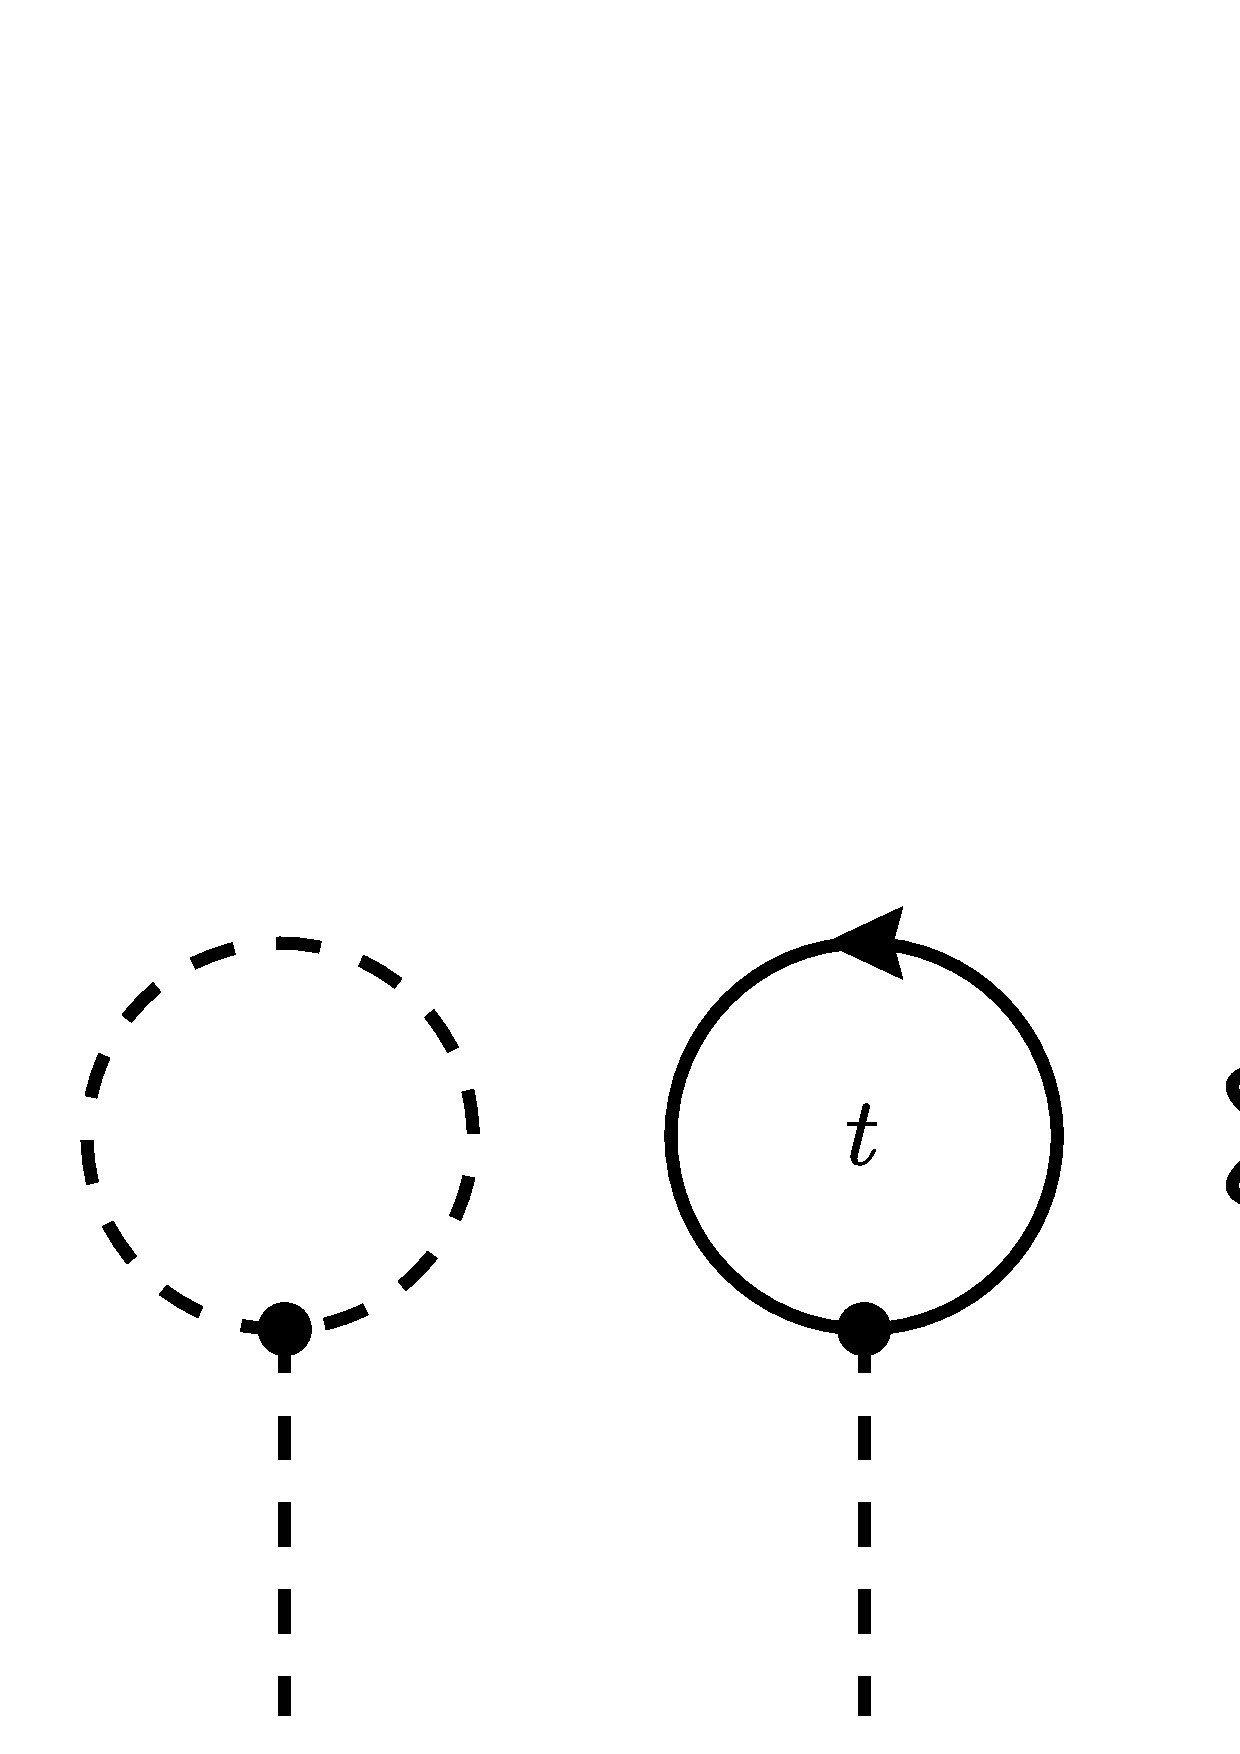
\includegraphics[scale=0.25]{Images/tadpoles.pdf}
\caption{Tadpole Feynman diagrams at one loop. All Feynman diagrams in this thesis were created using \texttt{FeynGame}~\cite{Harlander:2020cyh, Harlander:2024qbn, Bundgen:2025utt}.}
\label{fig:3:tadpoles}
\end{figure}
The factor $1/2$ is the symmetry factor of the diagram. According to Eq.~\eqref{eq:3:Veff_diff}, the effective potential can now be obtained through integration over $\omega$,
\begin{equation}
\begin{split}
V_\text{eff}^{(1)} &\big \vert_{\text{scalar}} =  \\
&\frac{\mu_R^{2 \epsilon}}{16 \pi^2} e^{\epsilon \gamma_E} \int \frac{\dd^d k}{i \pi^{d/2}} \int^{\phi} \dd \omega\, \frac{3 \lambda \omega}{k^2 - \mu^2 + 3 \lambda \omega^2} = \frac{\mu_R^{2 \epsilon}}{16 \pi^2} e^{\epsilon \gamma_E} \int \frac{\dd^d k}{i \pi^{d/2}} \frac{1}{2} \ln\! \left( \frac{k^2 - \mu^2 + 3 \lambda \phi^2}{k^2} \right).
\end{split}
\end{equation}
The lower bound of the $\omega$ integration is hereby irrelevant since it just results in a global shift of the potential. We chose the lower bound as $\sqrt{\mu^2/(3 \lambda)}$ in order to have a particularly easy $k$-integration. To solve the $k$-integral, we perform a \textit{Wick rotation} to Euclidean space, then the angular integration can be solved straightforwardly, resulting in
\begin{equation}
\begin{split}
V_\text{eff}\big \vert_{\text{scalar}} &= \frac{\mu_R^{2 \epsilon}}{16 \pi^2} e^{\epsilon \gamma_E} \int_0^\infty \dd k_E\, k_E^{d - 1}\ln\! \left(1 + \frac{\mu^2 - 3 \lambda \phi^2}{k_E^2} \right) \int_{\mathcal{S}_1^{d - 1}} \dd \Omega \frac{1}{2 \pi^{d/2}}  \\
& = \frac{\mu_R^{2 \epsilon}}{16 \pi^2} e^{\epsilon \gamma_E} \int_0^\infty \dd k_E\, k_E^{d - 1} \ln\! \left(1 + \frac{\mu^2 - 3 \lambda \phi^2}{k_E^2} \right) \frac{1}{\Gamma\! \left(\frac{d}{2} \right)} \\
&\hspace{-1.1mm}\stackrel{\text{IBP}}{=}  \frac{\mu_R^{2 \epsilon}}{16 \pi^2} e^{\epsilon \gamma_E} \frac{2}{\Gamma\! \left(\frac{d}{2} \right)} \int_0^\infty \dd k_E\, \frac{1}{d} k_E^{d - 1} \frac{\mu^2 - 3 \lambda \phi^2}{k_E^2 + \mu^2 - 3 \lambda \phi^2} \\
& =  \frac{\mu_R^{2 \epsilon}}{16 \pi^2} e^{\epsilon \gamma_E} \frac{1}{d \Gamma\! \left(\frac{d}{2} \right)} \left(\mu^2 - 3 \lambda \phi^2 \right)^{d/2} \int_0^\infty \dd x\, x^{\frac{d}{2} - 1} (1 + x)^{-1}
\end{split}
\end{equation}
In the third line we integrated by parts. The boundary terms can be set to zero in dimensional regularization since we can always find a dimension for which the integrand vanishes suitably fast (here $d \in (0, 2)$), and then use analytic continuation to generalize to arbitrary dimensions. In the last step, we substituted $x = k_E^2/(\mu^2 - 3 \lambda \phi^2)$. The resulting integral is \textit{Euler's $\beta$-function} $B\!\left(\frac{d}{2}, 1 - \frac{d}{2} \right)$. After expanding in $\epsilon$, we find that the effective potential is
\begin{equation}
V_{\text{eff}}\big \vert_{\text{scalar}} = \frac{(\mu^2 - 3 \lambda \phi^2)^2}{64 \pi^2} \left[ - \frac{1}{\epsilon} + \log\! \left( \frac{\mu^2 - 3 \lambda \phi^2}{\mu_R^2} \right) - \frac{3}{2} + \BigO{\epsilon} \right].
\end{equation}
As usual, the poles can be removed through renormalization. The contributions from fermions and the vector bosons are computed analogously. The full one-loop effective potential in the \MS\ scheme then reads
\begin{equation}
\begin{gathered}
V_\text{eff} = V_0 + V_1\\
V_0 = - \mu^2 \phi^2 + \lambda \phi^4, \quad V_1 = \sum_{i} \frac{n_i}{64 \pi^2} m_{i, \text{eff}}^4(\phi) \left[ \log\! \left( \frac{m_{i, \text{eff}}^2 (\phi)}{\mu_R^2} \right) - C_i \right],
\end{gathered}
\end{equation}
with $i = W,Z, t, H$ and
\begin{equation}
\begin{gathered}
C_W = C_Z = \frac{5}{6}, \quad C_t = C_H = \frac{3}{2}, \\
n_W = 6, \quad n_Z = 3, \quad n_t = -12, \quad n_H = 1, \\
m_{W, \text{eff}}^2 = \frac{1}{4} g_2^2 \phi^2, \quad m_{Z, \text{eff}}^2 = \frac{1}{4} \left(g_2^2 + g_Y^2 \right) \phi^2, \quad m_{t, \text{eff}}^2 = Y_t^2 \phi^2, \quad m_{H, \text{eff}}^2 = \mu^2 - 3 \lambda \phi^2.
\end{gathered}
\label{eq:3:Veff_params}
\end{equation}
Numerically, the top quark has the largest impact on the radiative corrections, with smaller but significant corrections coming from the vector bosons. The Higgs self coupling is only of minor significance, due to the small value of $\lambda$, and only becomes relevant at smaller field values, where the constant $\mu^2$-term can become important.

The $\mu^2 = 0$ case is particularly interesting because it represents the only dimensionful parameter in the \acs{SM} Lagrangian. If it could be set to zero, then the Lagrangian would be classically scale invariant, and all masses would be generated dynamically through radiative corrections. Models constructed under this assumption are call \textit{conformal models}. They were fairly popular a couple of decades ago since the additional scaling symmetry would also solve the electroweak hierarchy problem. If we assume $\mu^2 = 0$ and ignore the self-interaction of the Higgs, then the Higgs mass is easily calculable and reads
\begin{equation}
m_H^2 = \frac{3}{8 \pi^2}v^2 \left[ \frac{1}{16} (3 g_2^4 + 2 g_2^2 g_Y^2 + g_Y^4) - 4 Y_t^4 \right] .
\end{equation}
Unfortunately, the potential becomes unstable for top-quark masses above $125\ \mathrm{GeV}$, and hence the model is not realized in nature.

If we want to study the stability of the Higgs potential, then we must look at its behavior at large field values. At large $\phi$, logarithms of the form $\log (\phi^2/\mu_R^2)$ become large, and so our perturbative expansion becomes untrustworthy. To circumvent this, the appearing logarithms can be resummed to all orders by means of \acs{RGE} methods. The potential cannot depend on the unphysical renormalization scale, and hence must satisfy
\begin{equation}
0 = \frac{\dd V(\phi)}{\dd \log \mu_R} = \left( \frac{\partial}{\partial \log \mu_R} + \beta_\lambda \frac{\partial}{\partial \lambda} - \gamma_{\mu^2} \mu^2 \frac{\partial}{\partial \mu^2} - \gamma \phi \frac{\partial}{\partial \phi} + \sum_{i= 2, Y} \beta_i \frac{\partial }{\partial g_i} + \beta_{Y_t} \frac{\partial }{\partial Y_t} \right) V(\phi).
\label{eq:3:Veff_RGE}
\end{equation}
Here the $\beta$-funtions are defined as
\begin{equation}
\beta_\lambda = \frac{\dd \lambda}{\dd \log \mu_R}, \quad \beta_i = \frac{\dd g_i}{\dd \log \mu_R}.
\end{equation}
The anomalous dimensions of $\mu^2$ and the field, are
\begin{equation}
\gamma_{\mu^2} = - \frac{\dd \log \mu^2}{\dd \log \mu_R}, \quad \gamma = - \frac{\dd \log \phi}{\dd \log \mu_R}.
\end{equation}
The differential equation~\eqref{eq:3:Veff_RGE} can be solved via
\begin{equation}
\begin{gathered}
V (\phi) = -\frac{1}{2} \mu^2(t) G^2(t) \phi^2 + \frac{1}{4} \lambda(t) G^4(t) \phi^4, \quad t = \log\left( \frac{\phi}{\mu_R} \right), \\
G(t) \equiv \exp\! \left(- \int_0^t \dd t^\prime \ \gamma(g_i (t^\prime), \lambda (t^\prime)) \right).
\end{gathered}
\label{eq:3:Veff_solution}
\end{equation}
If instead, we expand \eqref{eq:3:Veff_RGE} in terms of couplings, we get
\begin{equation}
-\frac{\partial V_1(\phi)}{\dd \log \mu_R} = \left( \beta_\lambda \frac{\partial}{\partial \lambda} - \gamma_{\mu^2} \mu^2 \frac{\partial}{\partial \mu^2} - \gamma \phi \frac{\partial}{\partial \phi} + \sum_{i= 2, Y} \beta_i \frac{\partial }{\partial g_i} + \beta_{Y_t} \frac{\partial }{\partial Y_t} \right) V_0(\phi).
\end{equation}
Comparison of the quadratic and quartic terms then yieds expressions for $\beta_\lambda$ and $\gamma_{\mu^2}$
\begin{equation}
\begin{gathered}
\beta_\lambda = 4 \lambda \gamma + \frac{1}{16 \pi^2} (24 \lambda^2 + \frac{3}{2} g_2^4 + \frac{3}{8} (g_2^2 + g_Y^2)^2 - 24 Y_t^4), \\
\gamma_{\mu^2} = - 2 \gamma - \frac{3 \lambda}{4 \pi^2}.
\end{gathered}
\label{eq:3:beta_lambda_and_gamma_mu2}
\end{equation}
The Higgs anomalous dimension, can be easily derived from the two-point function. The result reads
\begin{equation}
\gamma = \frac{1}{64 \pi^2} \left( -9 g_2^2 - 3 g_Y^2 + 12 Y_t^2 \right).
\end{equation}
The remaining $\beta$-functions are
\begin{equation}
\begin{gathered}
\beta_{Y_t} = \frac{1}{16 \pi^2} \left(\frac{9}{2} Y_t^3 - 8 g_s^2 Y_t - \frac{9}{4} g^2 Y_t - \frac{17}{2} g_Y^2 Y_t \right), \quad \beta_s = - \frac{7}{16 \pi^2} g_s^3, \\
\beta_{g_2} = - \frac{19}{96 \pi^2} g_2^3, \quad \beta_{g_Y} = \frac{41}{96 \pi^2} g_Y^3.
\end{gathered}
\end{equation}
We thus obtained a system of differential equations for all the couplings. Once solved, the results can be inserted into~\eqref{eq:3:Veff_solution} to obtain the resummed effective potential. At one-loop the system of differential equations is already in a triangular form, meaning that the system of equations is already more or less decoupled. Furthermore, the \acs{RGE}s for $g_s, g_2$ and $g_Y$ are simple enough to be solved analytical. The results can then be inserted into the \acs{RGE} of $Y_t$, which is typically solved numerically. One then proceeds analogously with the \acs{RGE}s of $\lambda$ and $\mu^2$. The boundary conditions on the coupling constants can be set from measurements, whereas the boundary conditions on the $\mu^2$ and $\lambda$ are given by the requirement that
\begin{equation}
\frac{\dd V_{\text{eff}}}{\dd \phi}\bigg \vert_{\phi = v} = 0, \qquad \frac{\dd^2 V_\text{eff}}{\dd \phi^2} \bigg \vert_{\phi = v} = m_H^2.
\end{equation}
The renormalization scale dependence of the various couplings at one-loop accuracy are displayed in Fig.~\ref{fig:3:running_couplings}.

The resulting potential should now be accurate for very large field values, even reaching up to the \textit{Planck scale} if there is no beyond the \acs{SM} phyiscs entering in between. We can study the stability of the effective potential by studying its large $\phi$ limit at various scales. If we assume the \acs{SM} to be an accurate description of nature up to the Planck scale, then the effective potential should be bounded from below, or else the \acs{VEV} would not be stable. Furthermore, the effective potential can develop a second minimum. If this minimum has at a lower energy then our \acs{VEV}, then the universe would at some point in time transition from our current ``false'' vacuum to the true minimum of the potential. The various scenarios are illustrated in Fig.~\ref{fig:3:Veff_illustration}.
\begin{figure}[ht]
\centering
\includegraphics[scale=1.1]{Images/Veff_illustration.pdf}
\caption{Illustration of effective Higgs potential for various scenarios.}
\label{fig:3:Veff_illustration}
\end{figure}
In Fig.~\ref{fig:3:stability_scan}, we show the stability of the Higgs potential in the $(m_H, m_t)$ plane. We note that the stability bounds are notorious for being extremely sensitive to the chosen boundary conditions.
\begin{figure}[ht]
  \begin{minipage}[t]{0.48\textwidth}
  \centering
  \includegraphics[width=\textwidth]{Images/stability_scan.pdf}
  \captionof{figure}{Stability of the Higgs potential as a function of the Higgs and top-quark mass. Red areas are unstable, yellow areas are metastable, and green areas are stable. The computational setup described in the \hyperref[chap:notation_and_conventions]{Conventions}.}
  \label{fig:3:stability_scan}
  \end{minipage}
  \hspace{0.02\textwidth}
  \begin{minipage}[t]{0.48\textwidth}
  \centering
  \includegraphics[width=\textwidth]{Images/running_couplings.pdf}
  \captionof{figure}{Scale dependence at one-loop accuracy of the various couplings for the \acs{SM} values of the Higgs and top-quark mass. The computational setup described in the \hyperref[chap:notation_and_conventions]{Conventions}.}
  \label{fig:3:running_couplings}
  \end{minipage}
\end{figure}
We can see that due to the negative minus sign of the fermionic contributions to the effective potential (see $n_t$ in Eq.~\eqref{eq:3:Veff_params}), the potential becomes unstable if the top-quark mass becomes too large. We also observe that for the \acs{SM} Higgs and top-quark masses, the potential is unstable but very close to the stability bound. With a two-loop calculation, absolute stability is now excluded at the $3\sigma$-level~\cite{Degrassi:2012ry}. Since an unstable vacuum is impossible, there must be some new physics mechanism which ensures that the potential is bounded from below. If the new physics scale is smaller than the scale at which the quartic Higgs coupling becomes negative ($\sim 10^{12}\ \mathrm{GeV}$ see Fig.~\ref{fig:3:running_couplings}), then the potential would become absolutely stable once again. If, on the other hand, new physics only enters at even larger scales, then the potential exhibits a second \acs{VEV} and our universe is metastable.

If our vacuum is truly metastable, then a) there must be a mechanism which ensured that the correct ``false'' vacuum was chosen, and b) the false vacuum must be sufficiently stable to have survived for at least the age of our universe (13.8 billion years). The first point could for example be explained, if today's vacuum started of as the true vacuum and only became the false vacuum as the universe cooled down. How exactly the mechanism is realized is however highly model specific. The second point, that the false vacuum is sufficiently long-lived to have survived this long, is highly dependent on the new physics scale. Generally speaking, a higher new physics scale, results in a lower vacuum tunneling rate, that means the loosest bounds on \acs{SM} parameters are therefore derived assuming that new physics only enters at the Planck scale. Since the \acs{SM} is so close to the stability bound, it turns out that the Planck scale suffices to make the universe stable enough to have survived this long~\cite{Degrassi:2012ry}. To address the question posed at the beginning of this chapter regarding the stability of the Higgs potential: surprisingly, within the framework of the \acs{SM}, it is not stable. However, by making minimal assumptions about \acs{BSM} physics, there exists a vast parameter space where the \acs{VEV} is sufficiently stable to have persisted throughout the lifetime of the universe.

Lastly, we comment on the Landau pole of the quartic Higgs coupling. If $\beta_\lambda$ is positive, then $\lambda$ will at some point become large. If $\lambda$ approaches unity, we lose perturbative convergence, the $\beta_\lambda$ function will then become even larger and the Landau pole is quickly reached after losing perturbative convergence\footnote{Since the \acs{RGE} was derived perturbatively, it is, however, by no means clear that the pole would actually be reached.}. From  Eq.~\eqref{eq:3:beta_lambda_and_gamma_mu2}, we can see that the $\beta_\lambda$-function becomes larger for larger $\lambda$, ergo for larger Higgs-boson masses, but decreases for larger top-quark masses. For the \acs{SM} top-quark mass, one finds that the Higgs quartic coupling becomes non-perturbative at $m_H > 175\ \mathrm{GeV}$~\cite{Degrassi:2012ry}.

In conclusion, the Higgs boson is intricately connected to numerous fundamental concepts in physics, serving as a cornerstone in our understanding of particle interactions and symmetry breaking. Its properties not only illuminate aspects of the \acs{SM} but also offer valuable insights into \acs{BSM} theories. By examining the stability of the effective Higgs potential, we can impose significant constraints on both \acs{SM} and \acs{BSM} parameter spaces, guiding future research and deepening our comprehension of the universe's underlying principles.
